\documentclass{article}
\usepackage[utf8]{inputenc}
\usepackage{tikz}
\usetikzlibrary{shapes,shadows,arrows}

\tikzstyle{line} = [draw, -stealth, ultra thick]
\tikzstyle{elli}=[draw, ellipse, fill=white,minimum height=8mm, text width=9em, text centered]
\tikzstyle{block} = [draw, rectangle, text width=8em, text centered, minimum height=12mm, node distance=4.5em]
\tikzstyle{blockk} = [draw, rectangle, text width=8em, text centered, minimum height=12mm, node distance=5em]
\tikzstyle{block2} = [draw, rectangle, text width=10em, text centered, minimum height=15mm, node distance=9em]
\tikzstyle{block3} = [draw, rectangle, text width=20em, text centered, minimum height=15mm, node distance=13.5em]
\tikzstyle{block5} = [draw, rectangle, text width=22em, text centered, minimum height=15mm, node distance=7em]
\tikzstyle{block4} = [draw, rectangle, text width=10em, text centered, minimum height=15mm, node distance=7em]

\begin{figure}[t]
    \centering
    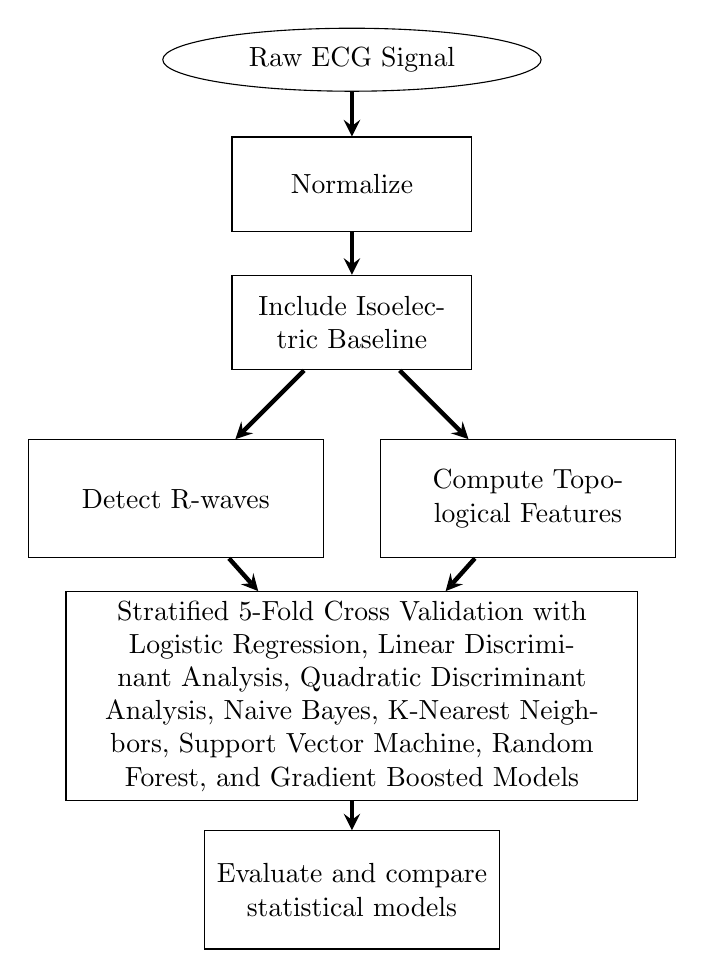
\begin{tikzpicture}
    \node [elli] (idx0) {Raw ECG Signal};
    \node [block, below of=idx0] (idx1) {Normalize};
    \node [blockk, below of=idx1] (idx2) {Include Isoelectric Baseline};
    \node [block2, below left of=idx2] (idx3) {Detect R-waves};
    \node [block2, below right of=idx2] (idx4) {Compute Topological Features};
    \node [block3, below of=idx2] (idx5) {Stratified 5-Fold Cross Validation with Logistic Regression, Linear Discriminant Analysis, Quadratic Discriminant Analysis, Naive Bayes, K-Nearest Neighbors, Support Vector Machine, Random Forest, and Gradient Boosted Models};
    \node [block4, below of=idx5] (idx6) {Evaluate and compare statistical models};
    \path [line] (idx0) -- (idx1);
    \path [line] (idx1) -- (idx2);
    \path [line] (idx2) -- (idx3);
    \path [line] (idx2) -- (idx4);
    \path [line] (idx3) -- (idx5);
    \path [line] (idx4) -- (idx5);
    \path [line] (idx5) -- (idx6);
    \end{tikzpicture}
    \caption{Flowchart of ECG Signal Processing and Arrhythmia Classification.}
    \label{fig:flowchart}
\end{figure}

